\section*{3.4 夹角与正交性}
\addcontentsline{toc}{section}{3.4 夹角与正交性}
\label{sec:3.4}

内积除了能够定义向量的长度以及两个向量之间的距离外，还可以通过定义两个向量之间的夹角 $ \omega $ 来刻画向量空间的几何性质。我们利用柯西-施瓦茨不等式~\eqref{eq:3-17} 来定义内积空间中两个向量 $ \boldsymbol{x}, \boldsymbol{y} $ 之间的夹角 $ \omega $，这一概念与我们在 $ \mathbb{R}^2 $ 和 $ \mathbb{R}^3 $ 中的直觉完全一致。假设 $ \boldsymbol{x} \neq \boldsymbol{0}, \boldsymbol{y} \neq \boldsymbol{0} $。则有：

\begin{equation}
-1 \leqslant \frac{\langle \boldsymbol{x}, \boldsymbol{y} \rangle}{\|\boldsymbol{x}\| \|\boldsymbol{y}\|} \leqslant 1
\tag{3.24}\label{eq:3-24}
\end{equation}

因此，存在唯一的 $ \omega \in [0, \pi] $（如图~\ref{fig:3-4} 所示），满足：

\begin{equation}
\cos \omega = \frac{\langle \boldsymbol{x}, \boldsymbol{y} \rangle}{\|\boldsymbol{x}\| \|\boldsymbol{y}\|}
\tag{3.25}\label{eq:3-25}
\end{equation}

数值 $ \omega $ 即为向量 $ \boldsymbol{x} $ 与 $ \boldsymbol{y} $ 之间的 \emph{夹角（angle）} 。直观上，两个向量之间的夹角反映了它们的方向有多相似。例如，使用点积时，$ \boldsymbol{x} $ 与 $ \boldsymbol{y} = 4\boldsymbol{x} $（即 $ \boldsymbol{y} $ 是 $ \boldsymbol{x} $ 的缩放版本）之间的夹角为 0：它们的方向是相同的。


\begin{figure}[H]
\centering
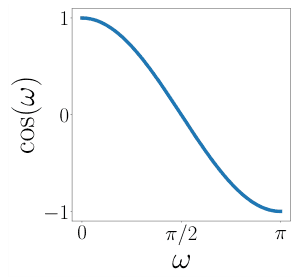
\includegraphics[width=0.92\textwidth,keepaspectratio]{docs/images/Figure3.4.png}
\caption*{\refstepcounter{figcounter}\label{fig:3-4}图~\thefigcounter 当限制在 [0, π] 上时，f(ω) = cos(ω) 在区间 [−1, 1] 内返回一个唯一的值。}
\end{figure}


\begin{notebox}
\textbf{例 3.6（向量之间的夹角）}
\end{notebox}

\begin{notebox}
让我们计算 $ \boldsymbol{x} = [1, 1]^\top \in \mathbb{R}^2 $ 与 $ \boldsymbol{y} = [1, 2]^\top \in \mathbb{R}^2 $ 之间的夹角；参见图~\ref{fig:3-5}，其中我们采用点积作为内积。由此可得：

\begin{equation}
\begin{adjustbox}{max width=\linewidth}
\cos \omega = \frac{\langle \boldsymbol{x}, \boldsymbol{y} \rangle}{\sqrt{\langle \boldsymbol{x}, \boldsymbol{x} \rangle \langle \boldsymbol{y}, \boldsymbol{y} \rangle}} = \frac{\boldsymbol{x}^\top \boldsymbol{y}}{\sqrt{\boldsymbol{x}^\top \boldsymbol{x} \boldsymbol{y}^\top \boldsymbol{y}}} = \frac{3}{\sqrt{10}}
\end{adjustbox}
\tag{3.26}\label{eq:3-26}
\end{equation}

这两个向量之间的夹角为 $ \arccos\left(\frac{3}{\sqrt{10}}\right) \approx 0.32\text{ rad} $，约合 $ 18^\circ $。
\end{notebox}


\begin{figure}[H]
\centering
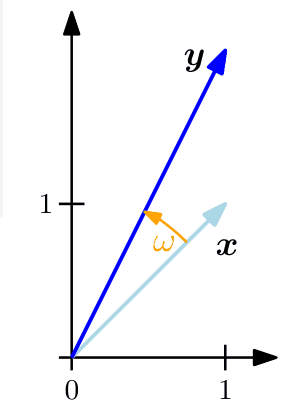
\includegraphics[width=320pt,keepaspectratio]{docs/images/Figure3.5.png}
\caption*{\refstepcounter{figcounter}\label{fig:3-5}图~\thefigcounter 两个向量 x, y 之间的夹角 ω 是通过内积计算的。}
\end{figure}


内积的一个关键特性在于，它还允许我们刻画正交的向量。

\textbf{定义 3.7}（正交性）。两个向量 $ \boldsymbol{x} $ 和 $ \boldsymbol{y} $ 是 \emph{正交的（orthogonal）} 当且仅当 $ \langle \boldsymbol{x}, \boldsymbol{y} \rangle = 0 $，我们记作 $ \boldsymbol{x} \perp \boldsymbol{y} $。如果此外还有 $ \|\boldsymbol{x}\| = 1 = \|\boldsymbol{y}\| $，即这两个向量是单位向量，则称 $ \boldsymbol{x} $ 和 $ \boldsymbol{y} $ 是 \emph{标准正交的（orthonormal）} 。

该定义的一个推论是，零向量与向量空间中的每一个向量都是正交的。

\emph{备注} 。正交性是将垂直概念推广到不一定为点积的双线性形式。在我们的语境中，从几何意义上讲，我们可以将正交向量看作关于特定内积成直角的向量。♦


\begin{figure}[H]
\centering
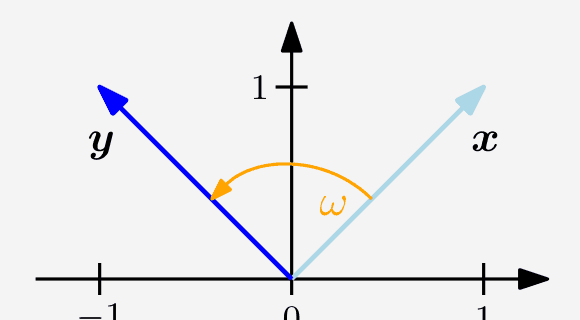
\includegraphics[width=0.92\textwidth,keepaspectratio]{docs/images/Figure3.6.png}
\caption*{\refstepcounter{figcounter}\label{fig:3-6}图~\thefigcounter 两个向量 x, y 之间的夹角 ω 会根据所选内积的不同而发生改变。}
\end{figure}


\begin{notebox}
\textbf{例 3.7（正交向量）}
\end{notebox}

\begin{notebox}
考虑两个向量 $ \boldsymbol{x} = [1, 1]^\top, \boldsymbol{y} = [-1, 1]^\top \in \mathbb{R}^2 $；参见图~\ref{fig:3-6}。我们希望使用两种不同的内积来确定它们之间的夹角 $ \omega $。以点积作为内积，得到 $ \boldsymbol{x} $ 与 $ \boldsymbol{y} $ 之间的夹角 $ \omega $ 为 $ 90^\circ $，从而 $ \boldsymbol{x} \perp \boldsymbol{y} $。然而，如果我们选择内积：

\begin{equation}
\langle \boldsymbol{x}, \boldsymbol{y} \rangle = \boldsymbol{x}^\top \begin{bmatrix} 2 & 0 \\ 0 & 1 \end{bmatrix} \boldsymbol{y}
\tag{3.27}\label{eq:3-27}
\end{equation}

则 $ \boldsymbol{x} $ 与 $ \boldsymbol{y} $ 之间的夹角 $ \omega $ 由下式给出：

\begin{equation}
\cos \omega = \frac{\langle \boldsymbol{x}, \boldsymbol{y} \rangle}{\|\boldsymbol{x}\| \|\boldsymbol{y}\|} = -\frac{1}{3} \implies \omega \approx 1.91\text{ rad} \approx 109.5^\circ
\tag{3.28}\label{eq:3-28}
\end{equation}

此时 $ \boldsymbol{x} $ 与 $ \boldsymbol{y} $ 并不正交。因此，关于某一种内积正交的向量，关于另一种不同的内积并不一定正交。
\end{notebox}

\textbf{定义 3.8}（正交矩阵）。方阵 $ \boldsymbol{A} \in \mathbb{R}^{n \times n} $ 是 \emph{正交矩阵（orthogonal matrix）} 当且仅当其列向量是标准正交的，从而满足：

\begin{equation}
\boldsymbol{A} \boldsymbol{A}^\top = \boldsymbol{I} = \boldsymbol{A}^\top \boldsymbol{A}
\tag{3.29}\label{eq:3-29}
\end{equation}

这蕴含着：

\begin{equation}
\boldsymbol{A}^{-1} = \boldsymbol{A}^\top
\tag{3.30}\label{eq:3-30}
\end{equation}

即逆矩阵只需通过对该矩阵进行转置即可得到。

\begin{notebox}
习惯上称这类矩阵为“正交矩阵”，但更精确的表述应该是“标准正交矩阵”。
\end{notebox}

由正交矩阵定义的变换十分特殊，因为向量 $ \boldsymbol{x} $ 在利用正交矩阵 $ \boldsymbol{A} $ 进行变换时其长度保持不变。对于点积，我们有：

\begin{equation}
\begin{adjustbox}{max width=\linewidth}
\|\boldsymbol{A} \boldsymbol{x}\|^2 = (\boldsymbol{A} \boldsymbol{x})^\top (\boldsymbol{A} \boldsymbol{x}) = \boldsymbol{x}^\top \boldsymbol{A}^\top \boldsymbol{A} \boldsymbol{x} = \boldsymbol{x}^\top \boldsymbol{I} \boldsymbol{x} = \boldsymbol{x}^\top \boldsymbol{x} = \|\boldsymbol{x}\|^2
\end{adjustbox}
\tag{3.31}\label{eq:3-31}
\end{equation}

\begin{notebox}
正交矩阵所对应的变换保持距离和夹角不变。
\end{notebox}

此外，利用内积度量的任意两个向量 $ \boldsymbol{x}, \boldsymbol{y} $ 之间的夹角，在同时使用正交矩阵 $ \boldsymbol{A} $ 对它们进行变换时也保持不变。假设以内积为点积，则像 $ \boldsymbol{A} \boldsymbol{x} $ 与 $ \boldsymbol{A} \boldsymbol{y} $ 之间的夹角由下式给出：

\begin{equation}
\begin{adjustbox}{max width=\linewidth}
\cos \omega = \frac{(\boldsymbol{A} \boldsymbol{x})^\top (\boldsymbol{A} \boldsymbol{y})}{\|\boldsymbol{A} \boldsymbol{x}\| \|\boldsymbol{A} \boldsymbol{y}\|} = \frac{\boldsymbol{x}^\top \boldsymbol{A}^\top \boldsymbol{A} \boldsymbol{y}}{\sqrt{\boldsymbol{x}^\top \boldsymbol{A}^\top \boldsymbol{A} \boldsymbol{x} \, \boldsymbol{y}^\top \boldsymbol{A}^\top \boldsymbol{A} \boldsymbol{y}}} = \frac{\boldsymbol{x}^\top \boldsymbol{y}}{\|\boldsymbol{x}\| \|\boldsymbol{y}\|}
\end{adjustbox}
\tag{3.32}\label{eq:3-32}
\end{equation}

这正好给出了 $ \boldsymbol{x} $ 与 $ \boldsymbol{y} $ 之间的夹角。这意味着满足 $ \boldsymbol{A}^\top = \boldsymbol{A}^{-1} $ 的正交矩阵 $ \boldsymbol{A} $ 既保持夹角不变，也保持距离不变。事实上，正交矩阵所定义的变换是旋转（可能伴随翻转）。在第 3.9 节中，我们将讨论有关旋转的更多细节。
